\documentclass{report}
\usepackage{pdfpages}
\usepackage{graphicx} 
\usepackage{dirtytalk}
\usepackage{lmodern}
\usepackage{booktabs}
\usepackage{listings}
\usepackage{float}
\usepackage{siunitx}
\usepackage{amsmath}
\usepackage{rotating}
\usepackage{arydshln}
\usepackage[hidelinks]{hyperref}
\usepackage[ngerman]{babel}
\usepackage[a4paper, total={6in, 8in}]{geometry}
\usepackage{caption}
\usepackage{amssymb}

\newcommand{\source}[1]{\caption*{Quelle: {#1}} }

\begin{document}
% 
\includepdf[pages=-]{./PDFs/Deckblatt_P2}
\begin{titlepage}
    \begin{center}
        \vspace*{1cm}
            
        \Huge
        \textbf{Auswertung und Protokoll}
            
        \vspace{0.5cm}
        \LARGE
        Zum Versuch ESK
        
        \vspace{1.8cm}

        \textbf{Jonas Müther \& Alejandro Schultheiss}
        \vfill
            
        P2 Praktikum\\
       
            
        \vspace{0.8cm}
  

        \vspace{1.8cm}
        \Large
        LMU München \\
        Physik B.Sc.\\
        Deutschland\\
        2026
            
    \end{center}
\end{titlepage}
\tableofcontents

\newpage
\chapter{Vorbereitung}

\section{Versuchsvorbereitung und Grundlagen des Versuchs}
% \includepdf[pages=-]{./PDFs/TEMP_VORBEREITUNG.pdf}

\section{Versuchsprotokoll}
% \includepdf[pages=-]{./PDFs/TEMP_VERSUCHSDURCHFUEHRUNG.pdf}

\newpage
\chapter{Auswertung}
\section{Teilversuch I: Belastungsabhängigkeit zweier Spannungsquellen}
In Teilversuch I sollte die Belastungsabhängigkeit zweier Spannungsquellen bestimmt werden.
Zur Bestimmung der Belastungsabhängigkeit wurde eine Schaltung nach folgendem Schaltplan aufgebaut.
\begin{figure}[H]
    \centering
    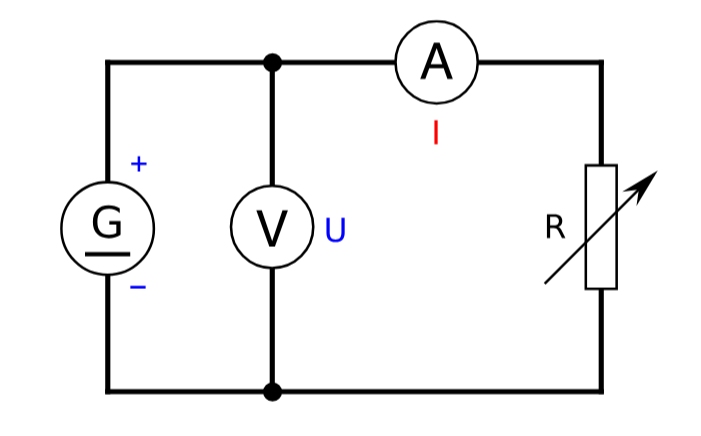
\includegraphics[width=0.5\textwidth]{./Images/TV1_Schaltplan.png}
    \caption{Schaltplan zur Bestimmung der Belastungsabhängigkeit verschiedener Spannungsquellen}
    \label{fig:SchemBelastAbh}
    \source{Abb. 26 der Versuchsanleitung zum Versuch ESK (P2-Praktikum der LMU München)}
\end{figure}
Die zwei verwendeten Spannungsquellen waren einerseits eine galvanische Zelle (Batterie) und andererseits ein Labornetzgerät. 
Während der Versuchsdurchführung wurden schrittweise die Potentiometereinstellungen variiert und dann die zugehörigen Ausgangsspannungen und Ströme gemessen.
\subsection{Galvanische Zelle}
Wir betrachten nun zunächst die galvanische Zelle. Für diese ergaben sich folgende Messwerte.
%INS Tabelle mit Ergebnissen einfügen

\newpage
\section{Teilversuch II: Bestätigung des Ohm'schen Gesetzes}
In Teilversuch II sollt das Ohm'sche Gesetz experimentell überprüft werden. Hierzu wurden nach folgendem Schaltplan Spannungen und Stromstärken durch einen Ohm'schen 
Widerstand gemessen. 
\begin{figure}[H]
    \centering
    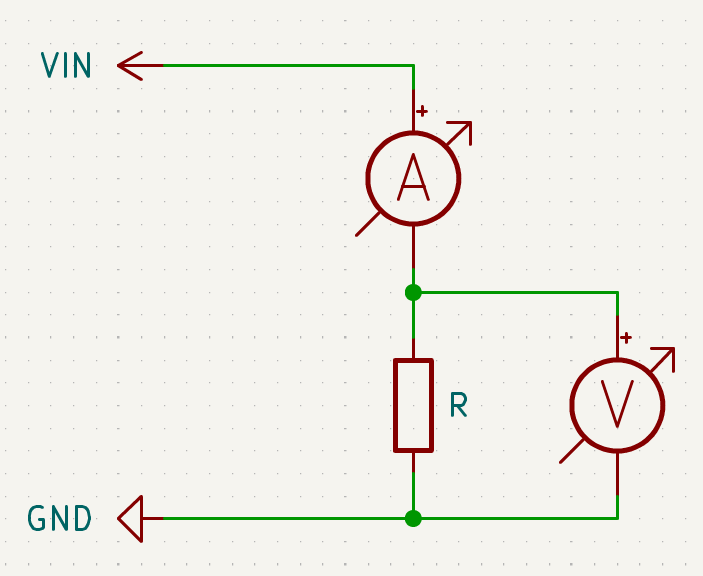
\includegraphics[width=0.5\textwidth]{./Images/TV2_Schaltplan.png}
    \caption{Schaltplan zur Messung von Strom und Spannung am Widerstand}
    \label{fig:SchemUIatR}
\end{figure}
Folgende Spannungs-Stromstärken-Wertepaare wurden gemessen:
%INS Werte eintragen
\begin{table}[H]
    \centering
    \caption{I-U-Tabelle eines Ohm'schen Widerstands}
    \label{tab:IUOhmscherWiderstand}
    \begin{tabular}{| c | c |}
        \hline
        Spannung $U$ in $\si{V}$ & Stromstärke $I$ in $\si{A}$ \\
        \hline
        $U1$ &  $I1$ \\
        \hline
        $U2$ &  $I2$ \\
        \hline
        $U3$ &  $I3$ \\
        \hline
        $U4$ &  $I4$ \\
        \hline
        $U5$ &  $I5$ \\
        \hline
        $U6$ &  $I6$ \\
        \hline
        $U7$ &  $I7$ \\
        \hline
        $U8$ &  $I8$ \\
        \hline
        $U9$ &  $I9$ \\
        \hline
        $U10$ &  $I10$ \\
        \hline
        $U11$ &  $I11$ \\
        \hline
    \end{tabular}
\end{table}
Diese Werte können nun mithilfe von Python und matplotlib geplottet werden. Damit erhält man folgenden Graphen:
%INS Plot einfügen

\newpage
\section{Teilversuch III: Spannungsabfall und Potentiometer}
\subsubsection{Spannungsabfall am stromdurchflossenen Draht}
\noindent
Durch den geraden Draht wurde ein näherungsweise konstanter Strom von

\begin{equation}
I=0{,}56\,\mathrm{A}
\end{equation}
\noindent
geschickt. Zunächst wurde der Spannungsabfall an drei verschiedenen
Drahtabschnitten gleicher Länge von jeweils $10\,\mathrm{cm}$ gemessen.

\begin{table}[htbp]
    \centering
    \caption{Spannungsabfall an verschiedenen Drahtabschnitten der Länge
    $10\,\mathrm{cm}$.}
    \label{tab:draht_10cm}
    \begin{tabular}{c|c}
        \hline
        Messung & $U$ in $\mathrm{V}$\\
        \hline
        1 & 0{,}67\\
        2 & 0{,}69\\
        3 & 0{,}69\\
        \hline
    \end{tabular}
\end{table}
\noindent
Der Mittelwert beträgt

\begin{equation}
\overline{U}_{10\,\mathrm{cm}}
=
\frac{0{,}67+0{,}69+0{,}69}{3}\,\mathrm{V}
=
0{,}683\,\mathrm{V}.
\end{equation}
\noindent
Die Messwerte unterscheiden sich nur geringfügig voneinander. Für einen
homogenen Draht wird bei gleicher Drahtlänge grundsätzlich derselbe
Spannungsabfall erwartet. Die kleinen Abweichungen können insbesondere durch
geringfügig unterschiedliche Kontaktpositionen sowie durch Kontaktwiderstände
zwischen Messspitzen und Draht hervorgerufen werden.
\noindent
Anschließend wurde der Spannungsabfall für verschiedene Drahtlängen bestimmt.

\begin{table}[htbp]
    \centering
    \caption{Spannungsabfall in Abhängigkeit von der Drahtlänge.}
    \label{tab:draht_laenge}
    \begin{tabular}{c|c}
        \hline
        $\Delta x$ in $\mathrm{cm}$ & $U$ in $\mathrm{V}$\\
        \hline
        20 & 1{,}38\\
        30 & 2{,}08\\
        40 & 2{,}76\\
        50 & 3{,}46\\
        60 & 4{,}13\\
        70 & 4{,}85\\
        \hline
    \end{tabular}
\end{table}
\noindent
Für einen homogenen Draht gilt

\begin{equation}
R=\rho\frac{L}{A}.
\end{equation}
\noindent
Mit dem Ohmschen Gesetz

\begin{equation}
U=RI
\end{equation}
\noindent
folgt bei konstantem Strom $I$ und konstantem Drahtquerschnitt

\begin{equation}
U
=
I\rho\frac{L}{A}
\end{equation}
\noindent
und damit

\begin{equation}
\boxed{U\propto L}.
\end{equation}
\noindent
Eine lineare Regression der Messwerte ergibt

\begin{equation}
U
=
0{,}06914\,\frac{\mathrm{V}}{\mathrm{cm}}
\cdot\Delta x
-
0{,}00143\,\mathrm{V}
\end{equation}
\noindent
mit

\begin{equation}
R^2=0{,}99994.
\end{equation}
\noindent
Der Achsenabschnitt liegt sehr nahe bei null und das Bestimmtheitsmaß ist
nahezu eins. Die gemessenen Werte bestätigen somit sehr gut die erwartete
lineare Abhängigkeit des Spannungsabfalls von der Drahtlänge.
\noindent
Aus der Steigung kann zusätzlich der Widerstand pro Längeneinheit des Drahtes
bestimmt werden. Mit $I=0{,}56\,\mathrm{A}$ ergibt sich

\begin{align}
\frac{R}{L}
&=
\frac{1}{I}\frac{\mathrm{d}U}{\mathrm{d}L}\\
&=
\frac{0{,}06914\,\mathrm{V/cm}}
{0{,}56\,\mathrm{A}}\\
&\approx
0{,}123\,\mathrm{\frac{\Omega}{cm}}.
\end{align}
\noindent
Dies entspricht

\begin{equation}
\frac{R}{L}
\approx
12{,}3\,\mathrm{\frac{\Omega}{m}}.
\end{equation}

\begin{figure}[htbp]
    \centering
    \        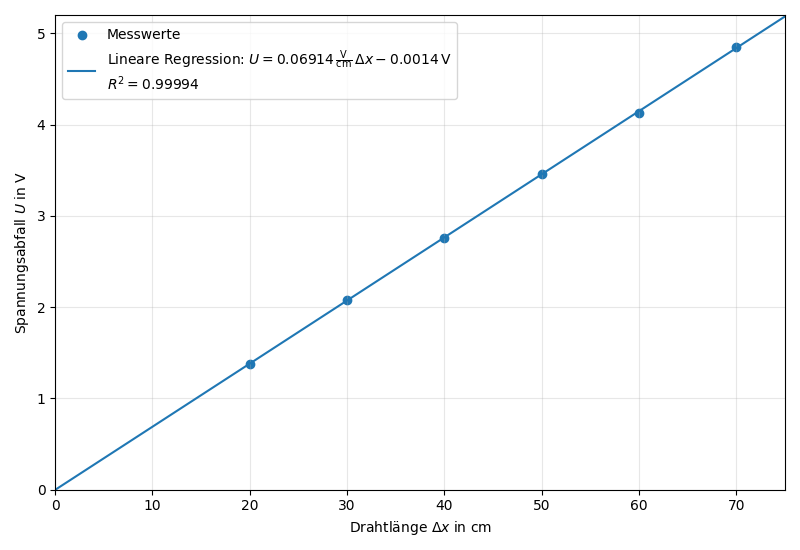
\includegraphics[width=0.5\textwidth]{./Images/TV3-1.png}

    \caption{Spannungsabfall am geraden Draht in Abhängigkeit von der
    betrachteten Drahtlänge.}
    \label{fig:draht_tv3}
\end{figure}


\subsubsection{Spannungsteilung am Wendelpotentiometer}
\noindent
Im zweiten Teil wurde die Ausgangsspannung eines Wendelpotentiometers in
Abhängigkeit von dessen Skalenstellung gemessen. Die am Potentiometer
angelegte Eingangsspannung betrug

\begin{equation}
U_0=10{,}10\,\mathrm{V}.
\end{equation}
\noindent
Die Messwerte sind in Tabelle~\ref{tab:helipot_tv3} dargestellt.

\begin{table}[htbp]
    \centering
    \caption{Ausgangsspannung des Wendelpotentiometers in Abhängigkeit
    von der Skalenstellung.}
    \label{tab:helipot_tv3}
    \begin{tabular}{c|c}
        \hline
        $x$ in Skt. & $U$ in $\mathrm{V}$\\
        \hline
        0    & 0{,}00\\
        100  & 1{,}001\\
        200  & 2{,}002\\
        300  & 3{,}00\\
        400  & 3{,}99\\
        500  & 4{,}99\\
        600  & 5{,}99\\
        700  & 7{,}90\\
        800  & 8{,}00\\
        900  & 9{,}00\\
        1000 & 10{,}00\\
        \hline
    \end{tabular}
\end{table}
\noindent
Für das Potentiometer gilt theoretisch

\begin{equation}
U
=
\frac{x}{x_0}U_0,
\end{equation}
\noindent
wobei $x_0=1000\,\mathrm{Skt.}$ der maximale Skalenwert ist. Somit wird eine
lineare Abhängigkeit der Ausgangsspannung von der Skalenstellung erwartet.
\noindent
Bei $U_0=10{,}10\,\mathrm{V}$ ergibt sich theoretisch

\begin{equation}
U(x)
=
0{,}01010\,\frac{\mathrm{V}}{\mathrm{Skt.}}\,x.
\end{equation}

\begin{figure}[htbp]
    \centering
        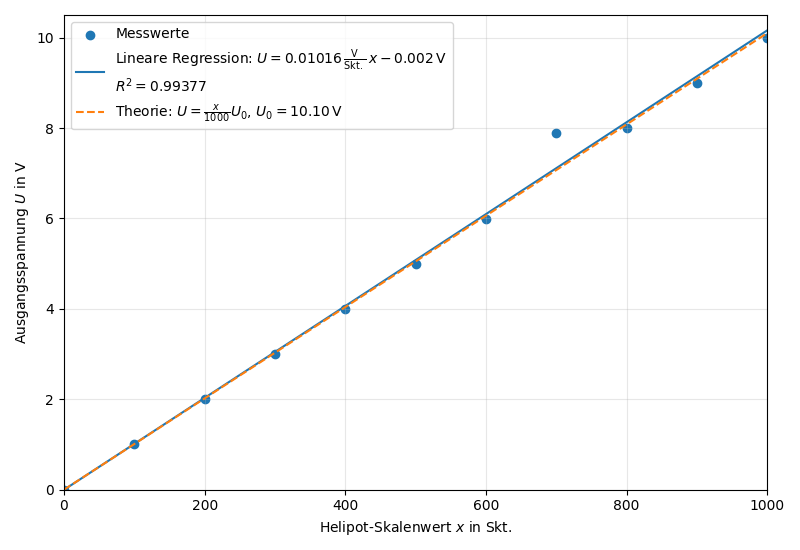
\includegraphics[width=0.5\textwidth]{./Images/TV3-2.png}
    \label{fig:helipot_tv3}
\end{figure}
\noindent
Die Messwerte zeigen mit Ausnahme des Messpunktes bei
$x=700\,\mathrm{Skt.}$ einen nahezu ideal linearen Verlauf. Für diesen
Skalenwert wurde

\begin{equation}
U(700)=7{,}90\,\mathrm{V}
\end{equation}
\noindent
gemessen. Nach dem theoretischen Zusammenhang wäre dagegen ungefähr

\begin{equation}
U_\mathrm{theo}(700)
=
\frac{700}{1000}\cdot10{,}10\,\mathrm{V}
=
7{,}07\,\mathrm{V}
\end{equation}
\noindent
zu erwarten.
\noindent
Der Messpunkt bei $700\,\mathrm{Skt.}$ weicht somit deutlich vom ansonsten
linearen Verlauf ab. Mit hoher Sicherheit, ist davon auszugehen, dass es sich hierbei um einen Dokumentationsfehler handelt; also human error.
\noindent
Eine lineare Regression unter Einbeziehung aller Messwerte ergibt

\begin{equation}
U
=
0{,}01016\,\frac{\mathrm{V}}{\mathrm{Skt.}}\,x
-
0{,}002\,\mathrm{V}
\end{equation}
\noindent
mit

\begin{equation}
R^2\approx0{,}9938.
\end{equation}
\noindent
Zur Beurteilung des ansonsten erkennbaren linearen Trends kann zusätzlich
betrachtet werden, wie sich die Messreihe ohne den auffälligen
$700$-Skt.-Messpunkt verhält. In diesem Fall ergibt sich

\begin{equation}
U
=
0{,}009999\,\frac{\mathrm{V}}{\mathrm{Skt.}}\,x
-
0{,}002\,\mathrm{V}
\end{equation}
\noindent
mit

\begin{equation}
R^2\approx0{,}999998.
\end{equation}
\noindent
Damit zeigt der übrige Datensatz die erwartete Proportionalität zwischen
Skalenstellung und Ausgangsspannung sehr deutlich.
\noindent
Auch die Endwerte stimmen näherungsweise überein: Bei maximaler
Helipotstellung wurde

\begin{equation}
U(1000)=10{,}00\,\mathrm{V}
\end{equation}
\noindent
gemessen, während die Eingangsspannung $U_0=10{,}10\,\mathrm{V}$ betrug.
Die verbleibende Differenz beträgt etwa $1\,\%$.


\subsubsection{Diskussion}
\noindent
Die Ergebnisse beider Versuchsteile lassen sich durch denselben physikalischen
Zusammenhang erklären. Bei konstantem Strom ist der Spannungsabfall proportional
zum Widerstand. Für einen homogenen Draht ist dessen Widerstand wiederum
proportional zur Drahtlänge. Daher steigt der Spannungsabfall am geraden Draht
linear mit der betrachteten Länge an.
\noindent
Beim Wendelpotentiometer wird mit zunehmender Skalenstellung ebenfalls ein
immer längerer Abschnitt des Widerstandsdrahtes abgegriffen. Dadurch steigt
der abgegriffene Widerstand und damit auch die Ausgangsspannung näherungsweise
linear an.
\noindent
Die Messung am geraden Draht bestätigt diesen Zusammenhang mit
$R^2=0{,}99994$ sehr gut. Auch das Wendelpotentiometer zeigt bis auf den
auffälligen Messwert bei $700\,\mathrm{Skt.}$ einen nahezu ideal linearen
Verlauf.
\noindent
Mögliche Ursachen für einzelne Abweichungen sind Kontaktwiderstände,
nicht exakt reproduzierbare Kontaktpositionen am Draht, Ablese- oder
Übertragungsfehler sowie die endliche Auflösung der verwendeten Messgeräte.
Insbesondere der Wert bei $700\,\mathrm{Skt.}$ ist mit dem Verlauf der
übrigen Messreihe nicht vereinbar und sollte daher als auffälliger Messpunkt
gekennzeichnet werden.
\noindent
Insgesamt bestätigen beide Versuchsteile die erwartete Proportionalität
zwischen der Länge eines homogenen Widerstandsdrahtes und dem an diesem
Abschnitt auftretenden Spannungsabfall.

\newpage
\section{Teilversuch IV: }

\newpage
\section{Teilversuch V: }
\noindent
In diesem Teilversuch wurden die Ströme und Spannungen in einem
Widerstandsnetzwerk gemessen und die beiden Kirchhoffschen Sätze überprüft.
\noindent
Nach der Knotenregel gilt für jeden Verzweigungspunkt

\begin{equation}
\sum I_\mathrm{zu}
=
\sum I_\mathrm{ab},
\end{equation}
\noindent
während nach der Maschenregel für jede geschlossene Masche

\begin{equation}
\sum_i U_i=0
\end{equation}
\noindent
gelten muss.

\subsubsection{Messunsicherheiten}
\noindent
Für die Strommessung war die Toleranz des Multimeters mit

\begin{equation}
\Delta I
=
1{,}0\,\%\cdot I + 5\,\mathrm{Digits}
\end{equation}
\noindent
auf dem laminierten Datenblatt angegeben.
\noindent
Da die Stromwerte mit einer Auflösung von $0{,}01\,\mathrm{mA}$ angezeigt
wurden, entsprechen fünf Digits

\begin{equation}
5\,\mathrm{Digits}=0{,}05\,\mathrm{mA}.
\end{equation}
\noindent
Damit gilt beispielsweise für $I=2{,}78\,\mathrm{mA}$

\begin{align}
\Delta I
&=
0{,}010\cdot2{,}78\,\mathrm{mA}
+
0{,}05\,\mathrm{mA}\\
&=
0{,}0778\,\mathrm{mA}.
\end{align}
\noindent
Gerundet ergibt sich somit

\begin{equation}
I=(2{,}78\pm0{,}08)\,\mathrm{mA}.
\end{equation}
\noindent
Analog ergeben sich für alle gemessenen Ströme:

\begin{table}[htbp]
    \centering
    \caption{Gemessene Ströme mit Multimeterunsicherheiten.}
    \label{tab:stroeme_tv5}
    \begin{tabular}{c|c}
        \hline
        Messposition & $I$ in $\mathrm{mA}$\\
        \hline
        $\nearrow$       & $2{,}78\pm0{,}08$\\
        $\triangledown$  & $1{,}32\pm0{,}07$\\
        $\otimes$        & $1{,}46\pm0{,}07$\\
        Spirale          & $1{,}46\pm0{,}07$\\
        $\triangle$      & $2{,}78\pm0{,}08$\\
        $\star$          & $1{,}32\pm0{,}07$\\
        $\square$        & $1{,}32\pm0{,}07$\\
        $\circ$          & $0{,}72\pm0{,}06$\\
        $\times$         & $0{,}58\pm0{,}06$\\
        \hline
    \end{tabular}
\end{table}
\noindent
Für die Spannungsmessung war einer Unsicherheit von 

\begin{equation}
\Delta U
=
0{,}9\,\%\cdot U+4\,\mathrm{Digits}
\end{equation}
\noindent
angegeben.
\noindent
Für $U_1$ und $U_3$ beträgt die letzte angezeigte Stelle
$0{,}001\,\mathrm{V}$, sodass vier Digits $0{,}004\,\mathrm{V}$
entsprechen. Für die übrigen Spannungen beträgt die Auflösung
$0{,}01\,\mathrm{V}$ und damit

\begin{equation}
4\,\mathrm{Digits}=0{,}04\,\mathrm{V}.
\end{equation}
\noindent
Damit ergeben sich

\begin{table}[htbp]
    \centering
    \caption{Gemessene Spannungen mit Multimeterunsicherheiten.}
    \label{tab:spannungen_tv5}
    \begin{tabular}{c|c}
        \hline
        Widerstand & $U$ in $\mathrm{V}$\\
        \hline
        $R_1$ & $1{,}948\pm0{,}022$\\
        $R_2$ & $9{,}96\pm0{,}13$\\
        $R_3$ & $1{,}948\pm0{,}022$\\
        $R_4$ & $2{,}88\pm0{,}07$\\
        $R_5$ & $5{,}12\pm0{,}09$\\
        \hline
    \end{tabular}
\end{table}


\subsubsection{Überprüfung der Knotenregel}
\noindent
Die Stromrichtung wird entsprechend der im Messprotokoll durch Pfeile eingezeichneten
Richtung gewählt.
\noindent
Am ersten Verzweigungspunkt gilt

\begin{equation}
I_{\triangle}
=
I_{\otimes}
+
I_{\triangledown}.
\end{equation}
\noindent
Mit den Messwerten folgt

\begin{equation}
2{,}78\,\mathrm{mA}
-
1{,}46\,\mathrm{mA}
-
1{,}32\,\mathrm{mA}
=
0{,}00\,\mathrm{mA}.
\end{equation}
\noindent
Die Knotenregel ist an diesem Punkt somit erfüllt.
\noindent
Am Verzweigungspunkt der beiden parallelen Widerstände $R_1$ und $R_3$
muss gelten

\begin{equation}
I_{\triangledown}
=
I_{\times}
+
I_{\circ}.
\end{equation}
\noindent
Es ergibt sich

\begin{align}
I_{\triangledown}
-
I_{\times}
-
I_{\circ}
&=
1{,}32-0{,}58-0{,}72\\
&=
0{,}02\,\mathrm{mA}.
\end{align}
\noindent
Die Abweichung von $0{,}02\,\mathrm{mA}$ ist deutlich kleiner als die
Messunsicherheiten der beteiligten Strommessungen. Die Knotenregel ist daher
auch hier mit den Messwerten vereinbar.
\noindent
Am Zusammenführungspunkt der beiden parallelen Zweige gilt entsprechend

\begin{equation}
I_{\times}+I_{\circ}=I_{\square}.
\end{equation}
\nonumber
Auch hier folgt

\begin{equation}
0{,}58+0{,}72-1{,}32
=
-0{,}02\,\mathrm{mA},
\end{equation}
\noindent
sodass die Knotenregel innerhalb der Messunsicherheit erfüllt ist.
\noindent
Im rechten unteren Zweig ergibt sich

\begin{equation}
I_{\square}=I_{\star},
\end{equation}
\noindent
also

\begin{equation}
1{,}32\,\mathrm{mA}
-
1{,}32\,\mathrm{mA}
=
0.
\end{equation}
\noindent
Am unteren Verzweigungspunkt gilt schließlich

\begin{equation}
I_{\nearrow}
=
I_{\mathrm{Sp}}
+
I_{\star},
\end{equation}
\noindent
wobei $I_{\mathrm{Sp}}$ den mit dem Spiralsymbol gekennzeichneten Strom
bezeichnet. Einsetzen liefert

\begin{equation}
2{,}78-1{,}46-1{,}32
=
0{,}00\,\mathrm{mA}.
\end{equation}
\noindent
Damit wird der erste Kirchhoffsche Satz an allen untersuchten
Verzweigungspunkten innerhalb der Messunsicherheiten bestätigt.


\subsubsection{Überprüfung der Maschenregel}
\noindent
Die Widerstände $R_1$ und $R_3$ liegen parallel. Daher muss für die kleine
Masche zwischen beiden Widerständen

\begin{equation}
U_1-U_3=0
\end{equation}
\noindent
gelten. Experimentell ergibt sich

\begin{equation}
1{,}948\,\mathrm{V}
-
1{,}948\,\mathrm{V}
=
0{,}000\,\mathrm{V}.
\end{equation}
\noindent
Die Maschenregel ist für diese Masche somit erfüllt.
\noindent
Für die Masche über $R_2$, $R_1$, $R_5$ und $R_4$ gilt

\begin{equation}
U_2-U_1-U_5-U_4=0.
\end{equation}
\noindent
Einsetzen ergibt

\begin{align}
U_2-U_1-U_5-U_4
&=
9{,}96
-
1{,}948
-
5{,}12
-
2{,}88\\
&=
0{,}012\,\mathrm{V}.
\end{align}
\noindent
Die Abweichung beträgt somit lediglich

\begin{equation}
12\,\mathrm{mV}.
\end{equation}
\noindent
Unter Berücksichtigung der Multimeterunsicherheiten ist dieser Wert mit null
vereinbar.
\noindent
Für die entsprechende Masche über $R_3$ ergibt sich

\begin{equation}
U_2-U_3-U_5-U_4=0
\end{equation}
\noindent
und damit ebenfalls

\begin{equation}
9{,}96
-
1{,}948
-
5{,}12
-
2{,}88
=
0{,}012\,\mathrm{V}.
\end{equation}
\noindent
Auch diese Maschengleichung ist daher innerhalb der Messunsicherheiten erfüllt.


\subsubsection{Berücksichtigung der Unsicherheiten}
\noindent
Zur quantitativen Beurteilung können die Unsicherheiten der Summen beziehungsweise
Differenzen kombiniert werden. Für die Masche

\begin{equation}
\Delta U_\mathrm{M}
=
U_2-U_1-U_5-U_4
\end{equation}
\noindent
ergibt sich bei quadratischer Kombination der einzelnen Beiträge

\begin{equation}
\Delta(\Delta U_\mathrm{M})
=
\sqrt{
(\Delta U_2)^2+
(\Delta U_1)^2+
(\Delta U_5)^2+
(\Delta U_4)^2
}.
\end{equation}
\noindent
Mit den ungerundeten Einzelunsicherheiten ergibt sich

\begin{equation}
\Delta(\Delta U_\mathrm{M})
\approx
0{,}18\,\mathrm{V}.
\end{equation}
\noindent
Damit folgt für die Maschensumme

\begin{equation}
\boxed{
\Delta U_\mathrm{M}
=
(0{,}01\pm0{,}18)\,\mathrm{V}
}.
\end{equation}
\noindent
Der Sollwert null liegt somit eindeutig innerhalb des Unsicherheitsintervalls.
\noindent
Für den Knoten an den beiden Parallelwiderständen ergibt sich entsprechend

\begin{equation}
\Delta I_\mathrm{K}
=
I_{\triangledown}
-I_{\times}
-I_{\circ}.
\end{equation}
\noindent
Die kombinierte Unsicherheit beträgt

\begin{equation}
\Delta(\Delta I_\mathrm{K})
=
\sqrt{
(\Delta I_{\triangledown})^2+
(\Delta I_{\times})^2+
(\Delta I_{\circ})^2
}
\approx
0{,}11\,\mathrm{mA}.
\end{equation}
\noindent
Damit erhält man

\begin{equation}
\boxed{
\Delta I_\mathrm{K}
=
(0{,}02\pm0{,}11)\,\mathrm{mA}
}.
\end{equation}
\noindent
Auch hier ist die beobachtete Abweichung vollständig mit null vereinbar.


\subsubsection{Diskussion}
\noindent
Der erste Kirchhoffsche Satz wird durch die gemessenen Ströme bestätigt.
Insbesondere ergibt sich für den Gesamtstrom

\begin{equation}
2{,}78\,\mathrm{mA}
=
1{,}46\,\mathrm{mA}
+
1{,}32\,\mathrm{mA},
\end{equation}
\noindent
während sich der Strom im Parallelzweig näherungsweise gemäß

\begin{equation}
1{,}32\,\mathrm{mA}
\approx
0{,}58\,\mathrm{mA}
+
0{,}72\,\mathrm{mA}
\end{equation}
\noindent
aufteilt.
\noindent
Auch der zweite Kirchhoffsche Satz wird bestätigt. An den parallel geschalteten
Widerständen $R_1$ und $R_3$ wurde mit jeweils $1{,}948\,\mathrm{V}$ dieselbe
Spannung gemessen. Für die größere Masche ergibt sich

\begin{equation}
U_1+U_4+U_5
=
9{,}948\,\mathrm{V},
\end{equation}

während an $R_2$

\begin{equation}
U_2=9{,}96\,\mathrm{V}
\end{equation}
\noindent
gemessen wurde. Die Differenz von nur $0{,}012\,\mathrm{V}$ ist wesentlich
kleiner als die kombinierte Messunsicherheit.
\noindent
Die kleinen verbleibenden Abweichungen können insbesondere durch die
Messunsicherheiten der Multimeter sowie deren endliche Innenwiderstände verursacht
werden. Bei einer Strommessung besitzt das Amperemeter einen von null verschiedenen
Innenwiderstand und verändert die Schaltung daher geringfügig. Ein Voltmeter besitzt
zwar einen hohen, aber ebenfalls endlichen Innenwiderstand und entnimmt einen kleinen
Messstrom.
\noindent
Insgesamt sind sämtliche überprüften Knoten- und Maschengleichungen innerhalb
der Messunsicherheiten mit den Kirchhoffschen Sätzen vereinbar. Die Messungen
bestätigen somit sowohl die Knotenregel als Ausdruck der Ladungserhaltung als
auch die Maschenregel als Folge der Energieerhaltung.







\newpage
\chapter{Anhang}
\section{Python Scripts}
Die Python Scripts, die zum Plotten der Grafiken verwendet wurden, wurden mit Unterstützung von KI erstellt und dann nach den eigenen Bedürfnissen weiter
bearbeitet.
\definecolor{codegreen}{rgb}{0,0.6,0}
\definecolor{codegray}{rgb}{0.5,0.5,0.5}
\definecolor{codepurple}{rgb}{0.58,0,0.82}
\definecolor{backcolour}{rgb}{0.95,0.95,0.92}

\lstdefinestyle{python}{
    backgroundcolor=\color{backcolour},   
    commentstyle=\color{codegreen},
    keywordstyle=\color{magenta},
    numberstyle=\tiny\color{codegray},
    stringstyle=\color{codepurple},
    basicstyle=\ttfamily\footnotesize,
    breakatwhitespace=false,         
    breaklines=true,                 
    captionpos=b,                    
    keepspaces=true,                 
    numbers=left,                    
    numbersep=5pt,                  
    showspaces=false,                
    showstringspaces=false,
    showtabs=false,                  
    tabsize=2
}

\end{document}
